\documentclass[conference]{IEEEtran}

\usepackage{tikz}

\usepackage[slovene]{babel}

% correct bad hyphenation here
\hyphenation{}

\begin{document}
	
	\title{Implementacija spletnega pajka}
	
	\author{Skupina \textbf{DOMACI-NJOKI}: Niki Bizjak, Bojan Vrangeloski, Uroš Škrjanc}


	
	\maketitle
	
	\begin{abstract}
		V poročilu o seminarski smo opisali strukturo našega spletnega pajka, njegovo delovanje in rezultate, ki smo jih dobili pri preizkušanju pajka.
	\end{abstract}
	
	\IEEEpeerreviewmaketitle
	
	\section{Uvod}
	
	Za prvo semianrsko nalogo pri predmetu Iskanje in ekstrakcija podatkov s spleta smo implemetirali spletnega pajka, ki je pregledal in v lokalno podatkovno bazo prenesel vsebino spletnih strani na štirih spletnih mestih (gov.si, evem.gov.si, e-uprava.gov.si, e-prostor.gov.si). V nadaljevanju poročila smo opisali strukturo in delovanje našega pajka, predstavili rezultate naše naloge in težave, na katere smo naleteli tekom dela.
	
	\section{Struktura pajka}
	
	Pajka smo izdelali v programskem jeziku Python. Strukturno je pajek razdeljen na tri med seboj povezane komponente, ki so v praogramski kodi definiani kot objekti:
	
	\begin{itemize}
		\item razhroščvealnik,
		\item pajek,
		\item shramba.
	\end{itemize}
	
	
	
	\begin{figure}[h]
		\centering
		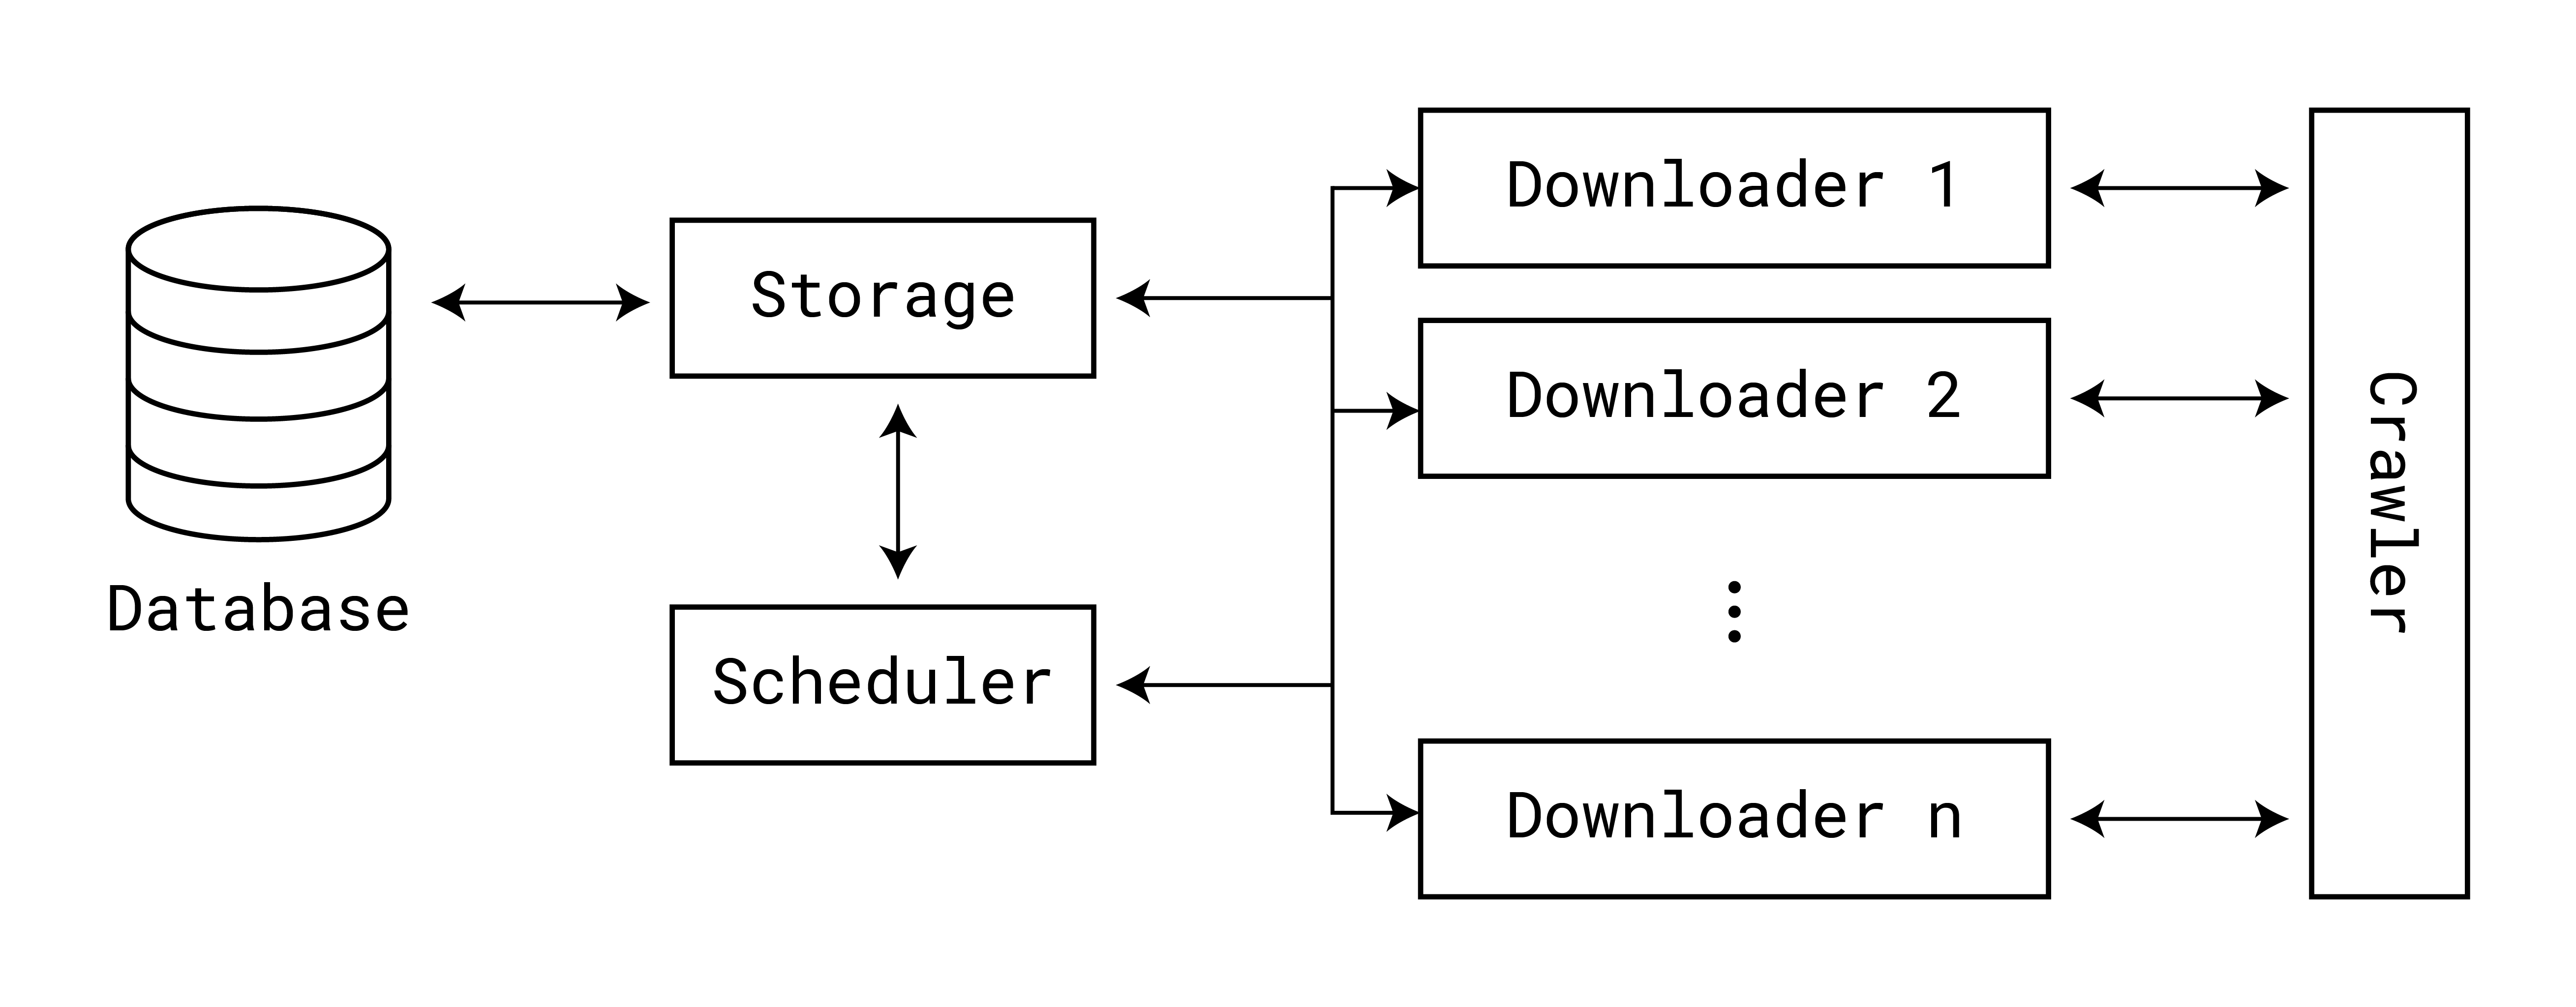
\includegraphics[width=.9\linewidth]{images/arhitecture}
		\caption{Arhitektura implementiranega spletnega pajka}
	\end{figure}

	\subsection{Razvrščevalnik}

	Razvrščevalnik (ang. scheduler) URL naslovov je implementiran kot podatkovna vrsta, do katere lahko obenem dostopa več različnih niti. 
	
	Ob dodajanju novega URL naslova v vrsto, razvrščevalnik preveri, ali je bil ta URL naslov že prenesen. Prav tako zna iz URL naslova prebrati domeno, pridobiti IP naslov strežnika s to domeno in prenesti datoteko \texttt{robots.txt}.
	
	\subsection{Pajek}
	
	Ob zagonu, pajek (ang. crawler) zažene več niti, vsaka od njih pa ima nalogo, da iz razvrščevalnika URL naslovov pridobi naslov, prenese stran in shrani podatke v podatkovno bazo. Pridobivanje vsebine strani izvajamo v dveh korakih:
	
	\begin{itemize}
		\item Najprej na strežnik izvedemo \texttt{HTTP HEAD} metodo.
		\item S pomočjo Selenium brskalnika obiščemo stran.
	\end{itemize}
	
	\subsection{Shramba}
	
	Shramba (ang. storage) je del pajka, ki skrbi za vpis zbranih podatkov in vsebin v relacijsko bazo podatkov. Baza je postavljena v okolju PostgreSQL, strukturi baze, ki je bila predlagana v projektu, pa smo v tabeli \texttt{page} dodali še polje \texttt{page hash}, v katerem se shranjuje hash vrednost, izračunana z MD5 algoritmom. Hash vrednost smo shranjevali za preverajnje, ali spletna stran z določeno vsebino že obstaja. 
	
	Za vpisovanje, popravljanje in izpis podatkov iz podatkovne baze smo sprogramirali 25 funkcij, vsaka od teh funkcij zaklene dostop do podatkovne baze, da ne bi prišlo do pomanjkljivih ali večkratnih vpisov vsebin.
	
	\section{Delo na projektu}
	
	Kar se tiče samega dela na projektu, je bilo najtežje uskladiti večnitno delovanje pajka in čakanje pri pošiljanju zahtev za spletne strani, tako da pajek deluje stabilno in hkrati v skaldu z etičnimi načeli. Vsaka takšna zahteva usklajeno delovanje tako med večimi nitmi samega pajka, kot tudi med vsemi komponentami, apliciranimi v pajku.
	
	\section{Rezultati}
	Naš spletni pajek je v ...urah zbral podatke o ... spletnih straneh, ... dokumentih in ... slikovnih datotekah. Glede na to, da gre za kar veliko količino podatkov, predvsem s kvantitativnega vidika, smatramo, da je delovanje pajka zadovoljivo. Tudi same podatke smo uspeli s spletnih mest pridobiti tako, da so primerni za nadajno uporabo, kar se nam zdi poembno za to nalogo. Je pa, seveda, tudi še nekaj prostora za izboljšave, ki bi jih lahko, če bi imeli na razplago nekaj več časa, tudi implementirali.
	
	V spodnji tabeli navajamo nekaj zanimivih rezultatov.

\begin{flushleft}
\begin{tabular}{ |l|l| } 
 \hline
 Število spletnih mest & ....  \\ 
 \hline
 Število speltnih strani & ...  \\  
 \hline
 Število dvojnikov strani & ... \\
 \hline
 Število dokumentov & ... \\
 \hline
 Število slik & ... \\
 \hline
 Povprečno število slik na stran & ... \\
 \hline
 Povprečno število dokumentov na stran & ... \\
 \hline
\end{tabular}
\end{flushleft}


	
	
	
	\section{Zaključek}
	
	
	
	% \bibliographystyle{IEEEtran}
	% \bibliography{}
	
\end{document}
